\section{LittlePanorama System}
\subsection{Overview}
In LittlePanorama, we implement the core features of Pan-orama in a simplified manner. One can think of LittlePan-orama as the lite version of Panorama. That said, at a high level, the design of LittlePanorama and Panorama are still much alike. 

\begin{figure}[!tb]
\centering
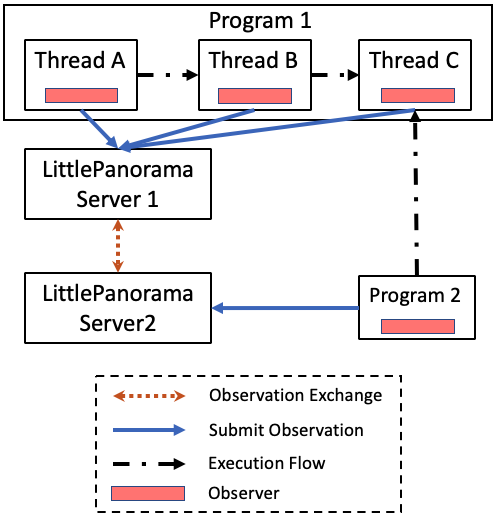
\includegraphics[width=\columnwidth]{figs/overview.png}
\vspace{-1em}
\caption{Overview of LittlePanorama
\label{fig:overview}
}
\end{figure}

Figure ~\ref{fig:overview} gives an overview of LittlePanorama. In a nutshell, LittlePanorama consists of two parts, LittlePanorama servers and observers. Each observer reports observations to a server on components it interacts with. Servers then make inference on whether one component has failed or not based on the observations received. They would also exchange observations such that all servers end up with the same set of observations. This idea of leveraging the interaction between components for failure detection is not new. Previous work ~\cite{van1998gossip} has employed similar ideas, but in a limited scope. By comparison, LittlePanorama (and of course Panorama) allows every component to report observations on any other component it interacts with. This gives LittlePanorama the ability to gather observations from a variety of perspectives. 

As a simple example, consider a program 1 in Figure ~\ref{fig:overview}. If only threads (in this case A, B and C) within program 1 could report observations on each other, it is unlikely that one would detect issues like network partition, as everything within program 1 remains functioning. However, if its peers, in this case program 2, could report observations on it, it would be easy to detect that program 1 is suffering from a network partition because program 1 would now become unreachable. Conversely, observers outside program 1 might not be able to report on the program's cpu/memory usage, and thus we would need observers within program 1 to detect if any thread is experiencing failures such as memory leak and cpu thrashing. 

Below we briefly discuss the key differences between the design of Panorama and LittlePanorama. 
\begin{itemize}
    \item \textbf{Where servers are located.} For each program monitored, a Panorama server instance would be colocated with it as its local storage for observations. In contrast, LittlePanorama servers are not colocated with any monitored program for simplicity. They are independent programs that may or may not run on the same machine as monitored programs.
    %\item \textbf{Whether a central inference server exists.} Panorama system has a central server that makes inference on a component based on observations received about it. In contrast, any LittlePanorama server would be able to make the inference.
    \item \textbf{How observers are created.} Both LittlePanorama and Panorama leverages code logic in existing components and make them observers. However, Panorama employs a static tool to automatically do so, while LittlePanorama does not have such a tool. Creating observers in LittlePanorama is done manually. Further details are provided in Section ~\ref{subsec:observers}.
    \item \textbf{Whether localizing failure is supported.} Besides deciding the status of a component, Panorama goes a step further by trying to localize a failure. To achieve this, Panorama introduces \textit{context}, a variable that describes what an observer is doing when it makes an observation. LittlePanorama does not have an implementation for \textit{context}.
    \item \textbf{The inference engine.} The authors report in the original paper that they use a bounded-look-back majority algorithm in their inference engine. We do not have a bound on the number of look-backs performed. More details are given in Section ~\ref{subsec:ie}.
\end{itemize}

\subsection{Abstractions and APIs}
One goal of LittlePanorama is to maintain the same abstraction and APIs as Panorama. Having the same APIs largely reduces the effort needed to reuse existing code from Panorama. In this section, we present terms and abstractions defined in the original paper ~\cite{huang2018capturing} with minor modification. 

Table ~\ref{tab:abs} lists the abstractions and terms that are used in both LittlePanorama and Panorama. A component is either a thread or a process. A component is an observer if it is capable of making observations on other components. Those that being observed are called subjects. In many cases, a component would be both an observer and a subject. Observations are sent to servers and stored there. 
%All servers are capable of making inference in LittlePanorama, while in Panorama there is a centralized inference server. 
Status defines the how healthy a component is and can only be one of eight pre-determined values, including HEALTHY and UNHEALTHY. One special value is PENDING, the use of which is beyond the scope of this project. More details can be found in the original paper. An observation contains information on a subject, which includes the identity of the observer and the subject, a timestamp and the observed status of the subject. 

Servers define a set of unified APIs for communicating with each other and observers. An example is ``SubmitObservation'', which is called by an observer to submit an observation. Other examples include ``RegisterObserver'', ``GetInference'' and ``ExchangeObservation''. Additional data structures and APIs are maintained by Panorama for enhanced functionalities. We consider them out-of-scope for this project. 

\begin{table}[!tb]
    \begin{tabular}{p{0.25\columnwidth}p{0.65\columnwidth}}%{l|l|l}
    
    \toprule    
    \textbf{Component}   &    a process or thread  \\
    \textbf{Subject}   &    a component to be monitored  \\ 
    \textbf{Observer}   &    a component monitoring a subject  \\
    \textbf{Server}   &    Panorama or LittlePanorama instance that receives observations and/or makes verdict  \\
    \midrule
    \textbf{Status}   &    the health situation of a subject  \\
    \textbf{Observation}   &  information an observer collects on a subject's status  \\
    \textbf{Inference}  &    a decision about a subject's status by summarizing a set of observations\\
    \bottomrule
    \end{tabular}
    \vspace{0.5em}
    \caption{Abstractions and terms used in LittlePanorama}
    \label{tab:abs}
\end{table}

\subsection{LittlePanorama Server}
LittlePanorama servers run independently as separate programs, while in Panorama they are colocated with monitored programs. Each LittlePanorama server has three key responsibilities: store all the observations sent to it, disseminate observations to other servers and make inference on the status of a subject using the inference engine described in Section ~\ref{subsec:ie}. It maintains an in-memory data structure map that saves all the observations made on each subject. The map is keyed by subject so that observations for a subject could be indexed efficiently. Unlike Panorama, we do not save anything to disk, which could be easily done with some engineering effort if we were to do it. Other differences between LittlePanorama and Panorama include whether to save all the observations or only n observations, whether a GC is implemented and whether to precompute an inference for each subject. We consider these differences to be of little importance. 

\subsection{Observers}
\label{subsec:observers}
One cool thing about Panorama is that it does not use any dedicated detectors. Instead, it turns existing components into observers by injecting API hooks into components' source code while keeping the functionalities unchanged. However, whenever an observer encounters an exception, it now not only handles it but also sends an observation through the API hooks. The process of adding hooks is done automatically in Panorama using a tool. 

Unfortunately, this tool is not published by the authors. We have to manually inject hooks. These hooks are generally injected at the boundaries between different components. In other words, hooks are expected to be injected in functions that switch between component. The authors give a brief guide on how to find these functions. It is still a challenging task without enough domain knowledge and time. In this project, we manually inject hooks to a few components without guaranteeing that they are injected at boundaries. 

That said, this does not mean that we are injecting hooks in the wrong way or in the wrong place. In fact, we inject hooks at near-boundaries. For example, ZooKeeper leader would ping its peers regularly. The boundary in this case would be the function that makes the RPC call and sends the ping packet to peers. Locating this function in thousands lines of code is nontrivial without enough domain knowledge. However, we could easily identify the function that initiates the ping request. We would then inject a hook into that function. 



\subsection{Observation Exchange}
In both Panorama and LittlePanorama, different observers might submit their observations on the same subject to different servers. To make sure that all servers see the same set of observations and thus making the same inference, a propagation protocol is used. Servers leverage this protocol to propagate/receive observations to/from each other. Besides this protocol, Panorama supports more sophisticated operations such as subscribing/unsubscribing to a subject. This is not implemented in LittlePanorama. Also, both Panorama and LittlePanorama assume a perfect network. Dealing with network failure is another research question of its own.

\subsection{Inference Engine}
\label{subsec:ie}
After collecting all the observations, an inference engine is used to decide the current status of a subject. The authors report in the original paper that they are using a bounded-look-back majority algorithm. When we implement it, we do not puts a bound on the number of look-backs performed. Our algorithm works as follows. 1. observations are grouped by observer. 2. for each group, observations are sorted in reverse chronological order. 3. we pick the status reported in the latest observation as the inference from this group. 4. we inspect observations from the latest to the oldest and average the scores reported in each observation. We stop when we hit an observation that reports a different status. 5. the status of a subject is determined via a majority vote across all the groups. Again, the authors' algorithm put a bound in step 4 while we do not.